\documentclass[]{usiinfprospectus}

\usepackage[utf8]{inputenc}
\usepackage[english]{babel}
\usepackage[T1]{fontenc}

\captionsetup{labelfont={bf}}

\author{Carlos Eduardo B. Bezerra}

\title{A fault tolerant multi-server system for MMOGs}
%\subtitle{A crash-stop model oriented approach}
\versiondate{\today}

\begin{committee}
%With more than 1 advisor an error is raised...: only 1 advisor is allowed!
\researchadvisor[Universit\`a della Svizzera Italiana, Switzerland]{Prof.}{Fernando}{Pedone}
\academicadvisor[Universit\`a della Svizzera Italiana, Switzerland]{Prof.}{Fernando}{Pedone}
\committeemember[Universit\`a della Svizzera Italiana, Switzerland]{Prof.}{Committee}{Member1}
\committeemember[Universit\`a della Svizzera Italiana, Switzerland]{Prof.}{Committee}{Member2}
%\committeemember[Universit\`a della Svizzera Italiana, Switzerland]{Prof.}{Committee}{Member3}
\coadvisor[Universidade Federal do Rio Grande do Sul, Brazil]{Prof.}{Cl\'audio}{Geyer}
%\coadvisor[Universit\`a della Svizzera Italiana, Switzerland]{Prof.}{Research}{Co-Advisor2}
%\coadvisor[Universit\`a della Svizzera Italiana, Switzerland]{Prof.}{Research}{Co-Advisor3}
\phddirector{Prof.}{Michele}{Lanza}
\end{committee}

\abstract {
Massively multiplayer online games have become, in the last decade, an important genre of online entertainment, having a significant market share. In these games, thousands to tens of thousands of participants play simultaneously with one another in the same match. However, traditionally, this kind of game is supported by a powerful (and expensive) central infrastructure with considerable cpu power and very fast and low latency Internet connections. This work proposes the use of a geographically distributed server system, formed by voluntary nodes which help serving the game to the players. Two very important features, therefore, must be provided: consistency (which may be week and only existing in the players' perspective) and fault tolerance, as some of the participating nodes may crash and become unavailable. For this work, we consider the crash-stop failure model.
}


\begin{document}
\maketitle

%%%%%%%%%%%%%%%%%%%%%%%%%
\section{Introduction} \label{sec_introduction}
%%%%%%%%%%%%%%%%%%%%%%%%%

all the mmog intro and context...

\subsection{Verbum Laudatur Si Factum Sequatur}

The research prospectus outlines the research area in which the student intends to perform research, and describes initial work performed by the student. It should be no more than 4 pages in length (excluding bibliography). The research prospectus must be submitted to the prospectus review committee at least one week before the {\em prospectus review}.

%%%%%%%%%%%%%%%%%%%%%%%%%
\section{Proposed Model} \label{sec:model}
%%%%%%%%%%%%%%%%%%%%%%%%%

This work considers persistent state real-time games with virtual environments where each player controls an avatar, which executes the commands issued by the player, hence interacting with the virtual world and with objects present in it, such as avatars of other players. The basic operation of the game network support system must be as follows: when a player connects to the server, it must send the current state of the player's avatar and of the surroundings of its current location; after that, this player keeps receiving periodic state updates for the objects which are relevant to it (usually, based on the the perceivability of such objects by the player [,]). When a player issues a command (such as to move its avatar from one place to the other, to pick up an object or to attack another player's avatar), it sends a message to the server containing such input, which is then processed by the server, which decides the outcome of this action, probably changing the state of the game, which is then broadcast to all involved players.

The next sections will describe the services the service must provide to the players connected to it (Section \ref{sec:services}), the specific requirements for a fault-tolerant distributed MMOG server system, considering the crash-stop failure model (Section \ref{sec:feats}), and the proposed distributed architecture (Section \ref{sec:arch}) and an algorithm devised to synchronize the game state between the replicas (Section \ref{sec:algorithm}). 

\subsection{Services to be provided} \label{sec:services}

As already mentioned, in order to provide the services required by the MMOG, this work proposes the use of a geographically distributed system composed of voluntary nodes working together to form a distributed MMOG server. This distributed server must deliver, at least, the following services:

\begin{itemize}
	\item \textbf{Simulation} of the game, that is, the receiving of actions sent by the players and then processing their corresponding outcomes, which may result in changes on the game state;
	\item \textbf{Broadcasting} of the current game state to the different players connected to it -- although sending the whole game state to every player is very likely unnecessary;
	\item \textbf{Storage} of the game's state, which is, in short, the combination of the states of each object in the virtual environment -- inanimate objects, players' avatars and ai-controlled characters (also know as non-playable characters, or NPCs);
	\item \textbf{Retrieval} of the state of each object in the game, so that whenever a player connects to a server, it may receive the current state of the game and then interact with a valid copy of the virtual environment.
\end{itemize}

It is important to note that in real-time games (as opposed to turn-based games), it is critical for the players to receive timely responses, that is, after issuing a command to the server, the time it takes for the new game state resulting from that command to arrive in the player's machine is short enough not to be an impediment to the game. In other words, there is a constraint on the time it takes for a player to see the result of each of his actions, in order to keep the game ``playable''. This applies specially to the situation where there are multiple players and it is desirable that each player is informed about the actions of others as soon as they happen, so that they can have a proper interaction. Therefore, although not every change in the game state is immediately important to every player, it is necessary to provide this \textbf{timeliness} for the delivery of state update messages to each player for at least a subset of the objects in the virtual environment. Usually, this subset consists of the objects which are perceivable by the player at each moment.

Besides the timeliness for the delivery of the messages, it is necessary to provide \textbf{consistency} for the game state between each pair of players interacting with one another, which means that, if two any players are interacting with each other or with the same object -- or, sometimes, even if they are just playing in the same location of the game's virtual environment --, the game state they perceive must be the same. Apart from that, another important requisite of multiplayer games is to provide \textbf{fairness}, in the sense that the outcome of the players' actions is decided according to the game rules and that none of the players has advantages over the others even if that implies a more complex message ordering algorithm, for example.


%%%%%%%%%%%%%%%%%%%%%%%%%
\subsection{Characteristics of the intended distributed game server system} \label{sec:feats}

The main purpose of the system is to reduce or, ideally, eliminate the necessity of a central server for the game. In this work, the approach proposed to achieve this is based on principles similar to those of volunteer computing, where a potentially large set of contributors make their computers available to perform tasks requested by some remote entity. With such a system, although each of these nodes is probably much less powerful than a traditional mmog server, when working together they can sum up the cpu power and network link necessary to host one of these games.

However, several questions arise when dealing with a potentially large scale geographically distributed server system composed of voluntary nodes. First, as the nodes are volunteer, there is no guarantee that they will be available whenever they are needed, neither there is any guarantee regarding the amount of resources that each of these nodes makes available for the system -- be it cpu power, network bandwidth or storage. Besides, not only can these nodes become unavailable, but there can be a high rate of nodes joining and leaving the system, characterizing churn. There are also problems related to the geographical distribution of this system, as the option of using efficient group communication techniques -- such as network level multicast -- is not widely available on the Internet.

Finally, considering the potentially large number of nodes in this system, it is very likely that some of them present failures, for what we are assuming the crash-stop failure model -- therefore, we assume the possibility of nodes crashing and network links becoming unavailable. The services provided by the system must continue even in the presence of such failures. Not only must the distribution itself be transparent to the players, but also the existence of failures and their countermeasures must not be noticeable by them.

%%%%%%%%%%%%%%%%%%%%%%%%%
\subsection{Proposed architecture} \label{sec:arch}

In order to split a game server into several smaller units executed by many volunteer nodes, it is used the idea of dividing the virtual environment in regions, each of which may be managed by a different server -- or set of server. There are many approaches proposed in the literature, such as using fixed size cells which are grouped into regions, or using binary space partition trees, and so on. For the sake of generality, the architecture proposed here  does not decide how exactly the partitioning of the virtual environment will be performed.

One of the assumptions here is that the events of the game lead to a deterministic resulting game state. In other words, if the game starts in the state $S_{a}$, there is only one possible state $S_{b}$ to be reached after a sequence $E=\{e_{1}, e_{2}, ..., e_{n}\}$ of events. So, the game state may be modeled as a state machine, which is replicated across the different game server nodes. These server nodes are divided in two categories: \textbf{region managers} and \textbf{region replicas}. Each region has only one manager, who is responsible for ordering the events that happen inside that region. The region replicas have no authority to order the events -- be it players' commands or non-player events, such as the actions of AI-controlled characters --, but they can deliver and process any event $e$, as long as the game state in their memory results from every game state \textit{causally} prior to $e$. We later present the causality definition considered here.

As proposed in [cite related work], it is used here the idea of \textbf{contact servers} and \textbf{target servers}. In our architecture, the players whose avatars are in a certain region are distributed among the server nodes responsible for that region. The distribution is decided based on the network latency for each pair client-server. Each client is assigned to a server to which it has the lowest network latency among all servers in its region. This server, to which the client communicates directly, is its contact server. The target server is always the region manager, which can also be the contact server for certain players. When one of the servers gets overloaded because of the broadcasting of messages to players, these messages are then sent via other routes, even if the network latency of that new route is higher. Figure \ref{fig:arch} illustrates this architecture.

\begin{figure}[!t]
	\centering
	\includegraphics[width=0.45\linewidth]{images/arch}
	\caption{Basic architecture with Region Managers and Region Replicas}
	\label{fig:arch}
\end{figure}



%%%%%%%%%%%%%%%%%%%%%%%%%
\subsection{Proposed causality definition and synchronization algorithm} \label{sec:algorithm}

When a player issues a command $c_{i}$, it is sent to its contact server, which forwards the command to the region manager. The region manager then processes the command sent by the player and calculates its resulting state, also considering every command -- or any kind of event -- $c_{j}$ sent by other players, such that $c_{j}$ was issued prior to $c_{i}$. Any prior event $c_{j}$ that the contact server should be aware of and that has not been received by the contact server of that player yet is then sent by the region manager. By having these prior events, the contact server is able to calculate the new game state that should be sent to the player who issued the command $c_{i}$.

The \textbf{causality} is defined here based on which objects are affected by an event. If commands $e_{i}$ and $e_{j}$ affect the same object, then they must be ordered. The order is defined by the time when they are delivered at the region manager responsible for that object.

asdf

We could also use the other idea (player --tob--> region servers; then region servers --lazy-synch-->all other servers)



%%%%%%%%%%%%%%%%%%%%%%%%%
começar a falar das características específicas do sistema servidor distribuído, o que ele deve fazer (replicação, sincronização, tolerância a falhas, modelo crash-stop)

when adding a large number of players (falar aqui de timeliness), specially if they are distributed among different servers, many questions become critical. (falar aqui da sincronização com vários servidores)

- direct communication (players -> signed -> check by servers OU )


As mentioned before, this work considers the crash-stop failure model. Therefore

%%%%%
\bibliographystyle{abbrv}
\bibliography{references}



\end{document}